\documentclass[aspectratio=169]{beamer}

% --- Theme ---
\usetheme{metropolis}
\usepackage{graphicx}
\usepackage{booktabs}
\usepackage{amsmath}
\usepackage{listings}

% --- Title Page Info ---
\title{Real-Time Light Dosimetry for Heritage Digital Twins}
\subtitle{via Texture Space Ray Tracing}
\date{July 2026}
\author{Duică Sebastian \\ Advisor: Assoc. Prof. Victor Ioan Bâcu}
\institute{Technical University of Cluj-Napoca \\ Faculty of Automation and Computer Science}

\begin{document}

% --- Slide 1: Title Slide ---
\begin{frame}
    \titlepage
\end{frame}

% --- Slide 2: Agenda ---
\begin{frame}{Content}
    \begin{itemize}
        \item Context and Motivation
        \item Objectives
        \item Related Work
        \item Architecture and Solution
        \item Experiments and Validation
        \item Conclusions
    \end{itemize}
\end{frame}

% --- Slide 3: Context and Motivation ---
\begin{frame}{Context and Motivation}
    \begin{itemize}
        \item \textbf{Context:} Museum artifacts suffer irreversible photometric damage from cumulative light exposure over time.
        \item \textbf{Motivation:} Physical lux meters are spatially limited and cannot predict future damage under changing environmental conditions.
        \item \textbf{Need:} A highly scalable Digital Twin capable of simulating an entire 8,760-hour yearly cycle.
    \end{itemize}
\end{frame}

% --- Slide 4: Objectives ---
\begin{frame}{Objectives}
    \begin{itemize}
        \item \textbf{Main Objective:} To study, design, and implement a real-time metrology digital twin using Texture Space Ray Tracing.
        \item \textbf{Secondary Objectives:}
              \begin{itemize}
                  \item Integrate astronomical equations for solar ephemeris.
                  \item Implement the Perez All-Weather Sky Model for indirect light.
                  \item Evaluate the impact of architectural conservation scenarios.
              \end{itemize}
    \end{itemize}
\end{frame}

% --- Slide 5: Related Work ---
\begin{frame}{Related Work}
    \begin{table}[]
        \centering
        \resizebox{\textwidth}{!}{%
            \begin{tabular}{lll}
                \toprule
                \textbf{Reference}       & \textbf{Description}       & \textbf{Advantage/Disadvantage}                     \\ \midrule
                Pharr et al. (PBRT)      & Physically Based Rendering & Foundation of light transport mathematics           \\
                Veach \& Guibas          & Monte Carlo Integration    & Highly accurate, but computationally expensive      \\
                Perez et al.             & Sky Luminance Distribution & Predicts realistic cloudy/clear sky ratios          \\
                Traditional Screen-Space & Rasterization Techniques   & Fast, but fails with off-screen geometric occlusion \\ \bottomrule
            \end{tabular}%
        }
    \end{table}
\end{frame}

% --- Slide 6: Solution Overview ---
\begin{frame}{Solution Overview: System Architecture}
    \begin{columns}[c]
        \begin{column}{0.45\textwidth}
            \centering
            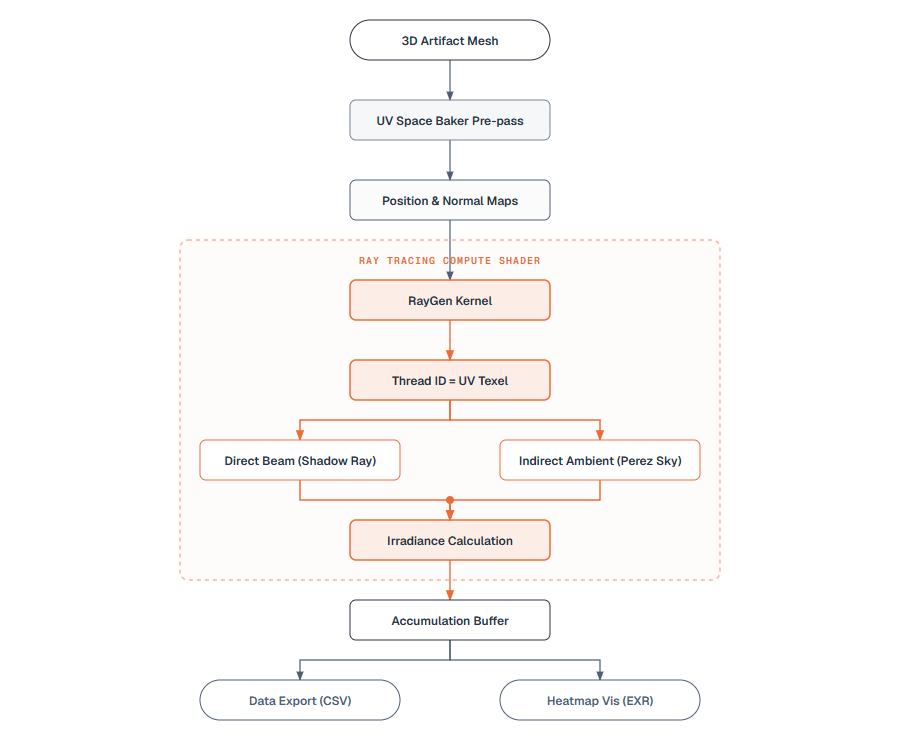
\includegraphics[width=\textwidth,keepaspectratio]{figures/pipeline.png}
        \end{column}
        \begin{column}{0.5\textwidth}
            \begin{itemize}
                \item \textbf{The Core Pipeline:} C\# orchestrates the celestial telemetry on the CPU, while the hardware-accelerated DirectX 12 GPU executes the path tracing.
            \end{itemize}
        \end{column}
    \end{columns}
\end{frame}

% --- Slide 6b: Detailed Architecture ---
\begin{frame}{Solution Overview: Detailed Architecture}
    \centering
    
\includegraphics[height=0.7\textheight]{figures/architecture.png}
\end{frame}

% --- Slide 7: Astrometric Orchestration ---
\begin{frame}{Solution: Astrometric Orchestration}
    \begin{itemize}
        \item \textbf{C\# CPU Thread:} Decoupled from the rendering engine to prevent viewport freezing.
        \item \textbf{Julian Day Math:} Converts the 8,760-hour cycle into exact geospatial sun altitudes and azimuths.
        \item \textbf{Result:} A completely deterministic, geographically synchronized solar vector for the GPU.
    \end{itemize}
\end{frame}

% --- Slide 8: Texture Space Path Tracer ---
\begin{frame}{Solution: Texture Space Path Tracer}
    \begin{columns}[c]
        \begin{column}{0.45\textwidth}
            \centering
            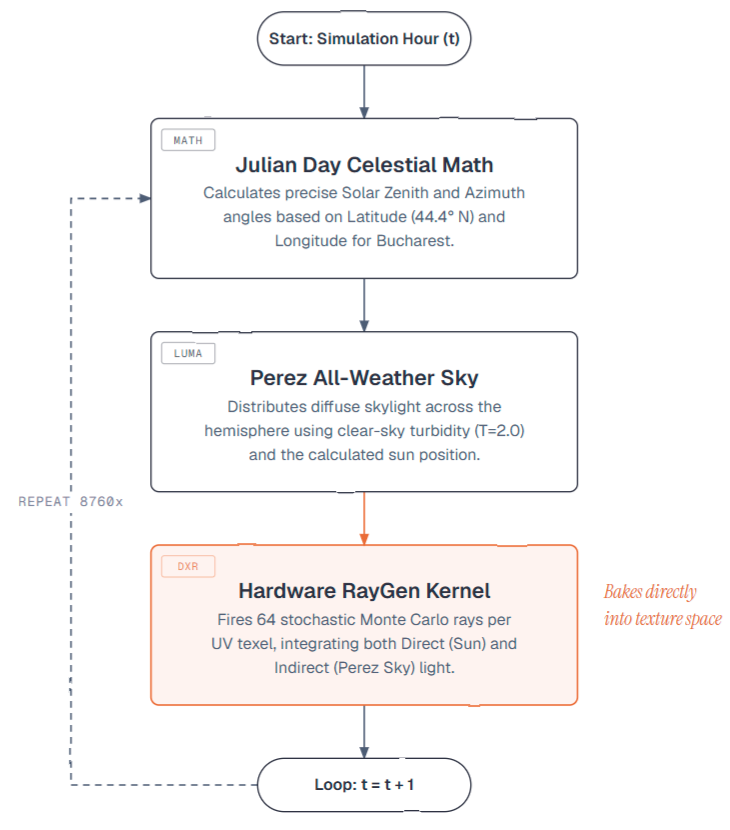
\includegraphics[width=\textwidth,height=0.85\textheight,keepaspectratio]{figures/astrometric_flowchart.png}
        \end{column}
        \begin{column}{0.5\textwidth}
            \begin{itemize}
                \item \textbf{Bypassing Screen Space:} By baking directly into the artifact's UV maps, we ensure perfect geometric occlusion even when the camera looks away.
            \end{itemize}
        \end{column}
    \end{columns}
\end{frame}

% --- Slide 9: Ambient Skylight ---
\begin{frame}{Solution: Ambient Skylight}
    \begin{itemize}
        \item \textbf{Perez All-Weather Model:} Simulates realistic relative luminance distribution on the sky dome (Clear Sky, $T=2.0$).
        \item \textbf{Cosine-Weighted Importance Sampling:} Stochastic multi-sampling concentrates rays toward the zenith, dramatically reducing variance.
    \end{itemize}
\end{frame}

% --- Slide 10: Data Telemetry ---
\begin{frame}{Solution: Data Telemetry}
    \centering
    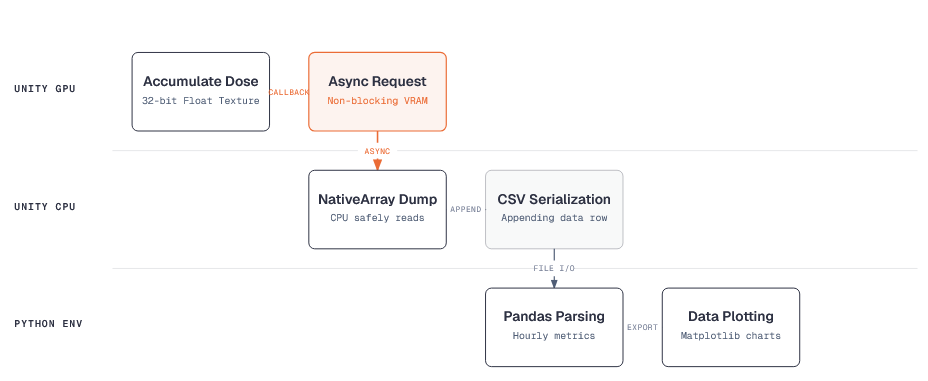
\includegraphics[width=\textwidth]{figures/telemetry_swimlane.png}
    \vspace{0.5cm}
    \begin{itemize}
        \item \textbf{Asynchronous Readback:} Ensures that extracting the 32-bit float accumulation buffers to CSV does not stall the GPU pipeline.
    \end{itemize}
\end{frame}

% --- Slide 11: Experimental Setup ---
\begin{frame}{Experiments and Validation: Setup}
    \begin{columns}[c]
        \begin{column}{0.5\textwidth}
            \begin{itemize}
                \item \textbf{Asset:} The Stanford Bunny, geometrically normalized and centered.
                \item \textbf{Location:} Bucharest, Romania.
                \item \textbf{Hardware:} NVIDIA RTX 4070 Ti Super (DX12 DXR).
                \item \textbf{Simulation Duration:} One full meteorological year (8,760 hours).
            \end{itemize}
        \end{column}
        \begin{column}{0.5\textwidth}
            \centering
            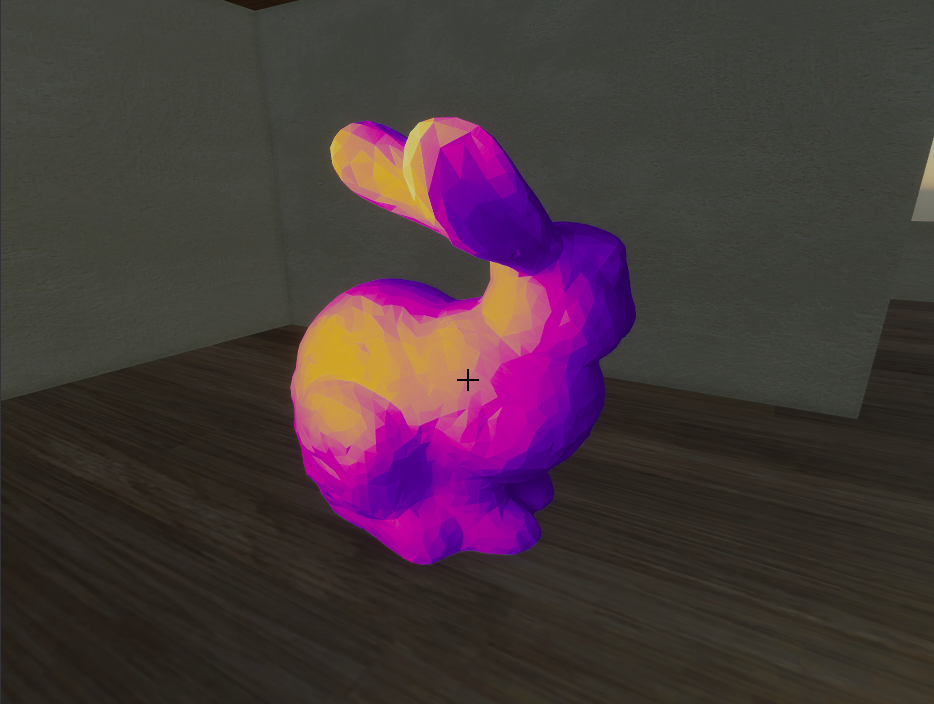
\includegraphics[width=\textwidth,keepaspectratio]{figures/fig_heatmap_visualisation.png}
        \end{column}
    \end{columns}
\end{frame}

% --- Slide 12: Conservation Scenarios ---
\begin{frame}{Experiments: Conservation Scenarios}
    \begin{table}[]
        \centering
        \begin{tabular}{ll}
            \toprule
            \textbf{Scenario} & \textbf{Intervention Description}                           \\ \midrule
            A (Baseline)      & Direct southern window exposure, standard materials.        \\
            B (Materials)     & UV-filtering glass and matte architectural floor applied.   \\
            C (Position)      & Artifact moved to a shaded corner, preventing direct sun.   \\
            D (Synergy)       & Both UV-filtering materials and corner positioning applied. \\ \bottomrule
        \end{tabular}
    \end{table}
\end{frame}

% --- Slide 13: Results - Diurnal Exposure ---
\begin{frame}{Experimental Results: Diurnal Exposure}
    \centering
    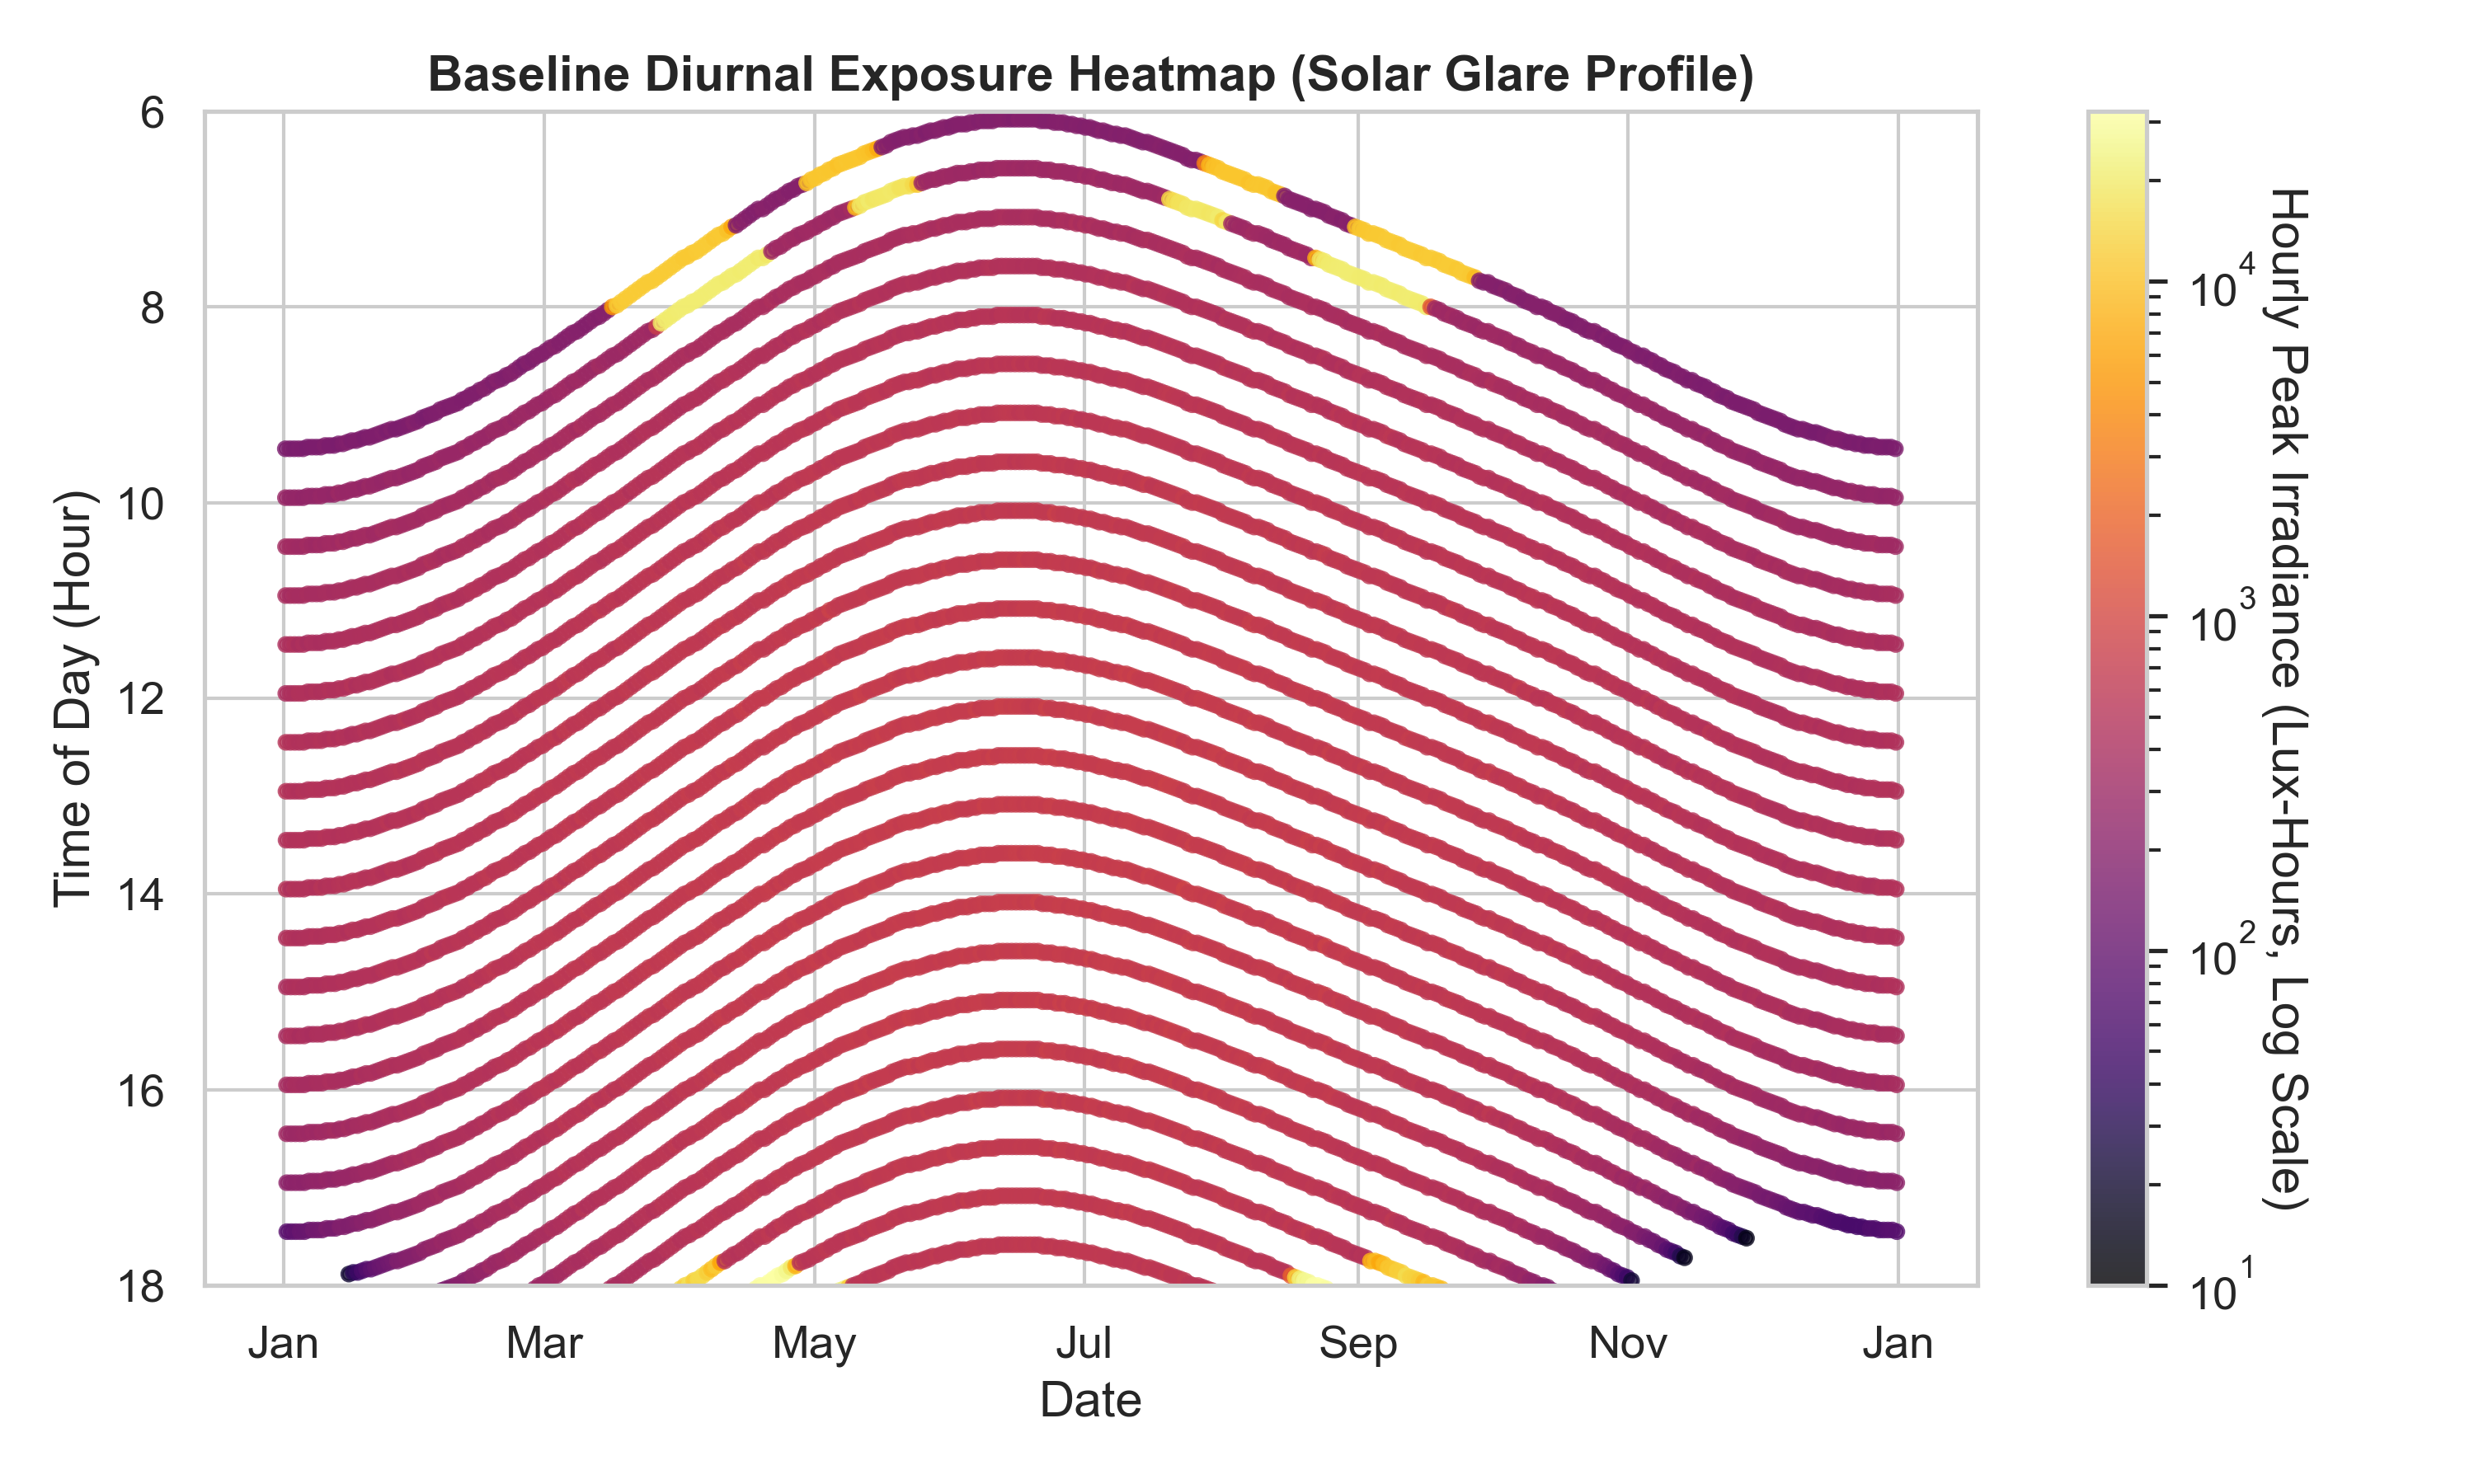
\includegraphics[height=0.6\textheight]{figures/fig4_diurnal_heatmap.png}
    \vspace{0.5cm}
    \begin{itemize}
        \item \textbf{Solar Glare Profile:} High concentration of irradiance precisely traces the sun's path during the summer months.
    \end{itemize}
\end{frame}

% --- Slide 14: Results - Final Dose ---
\begin{frame}{Experimental Results: Final End-of-Year Dose}
    \centering
    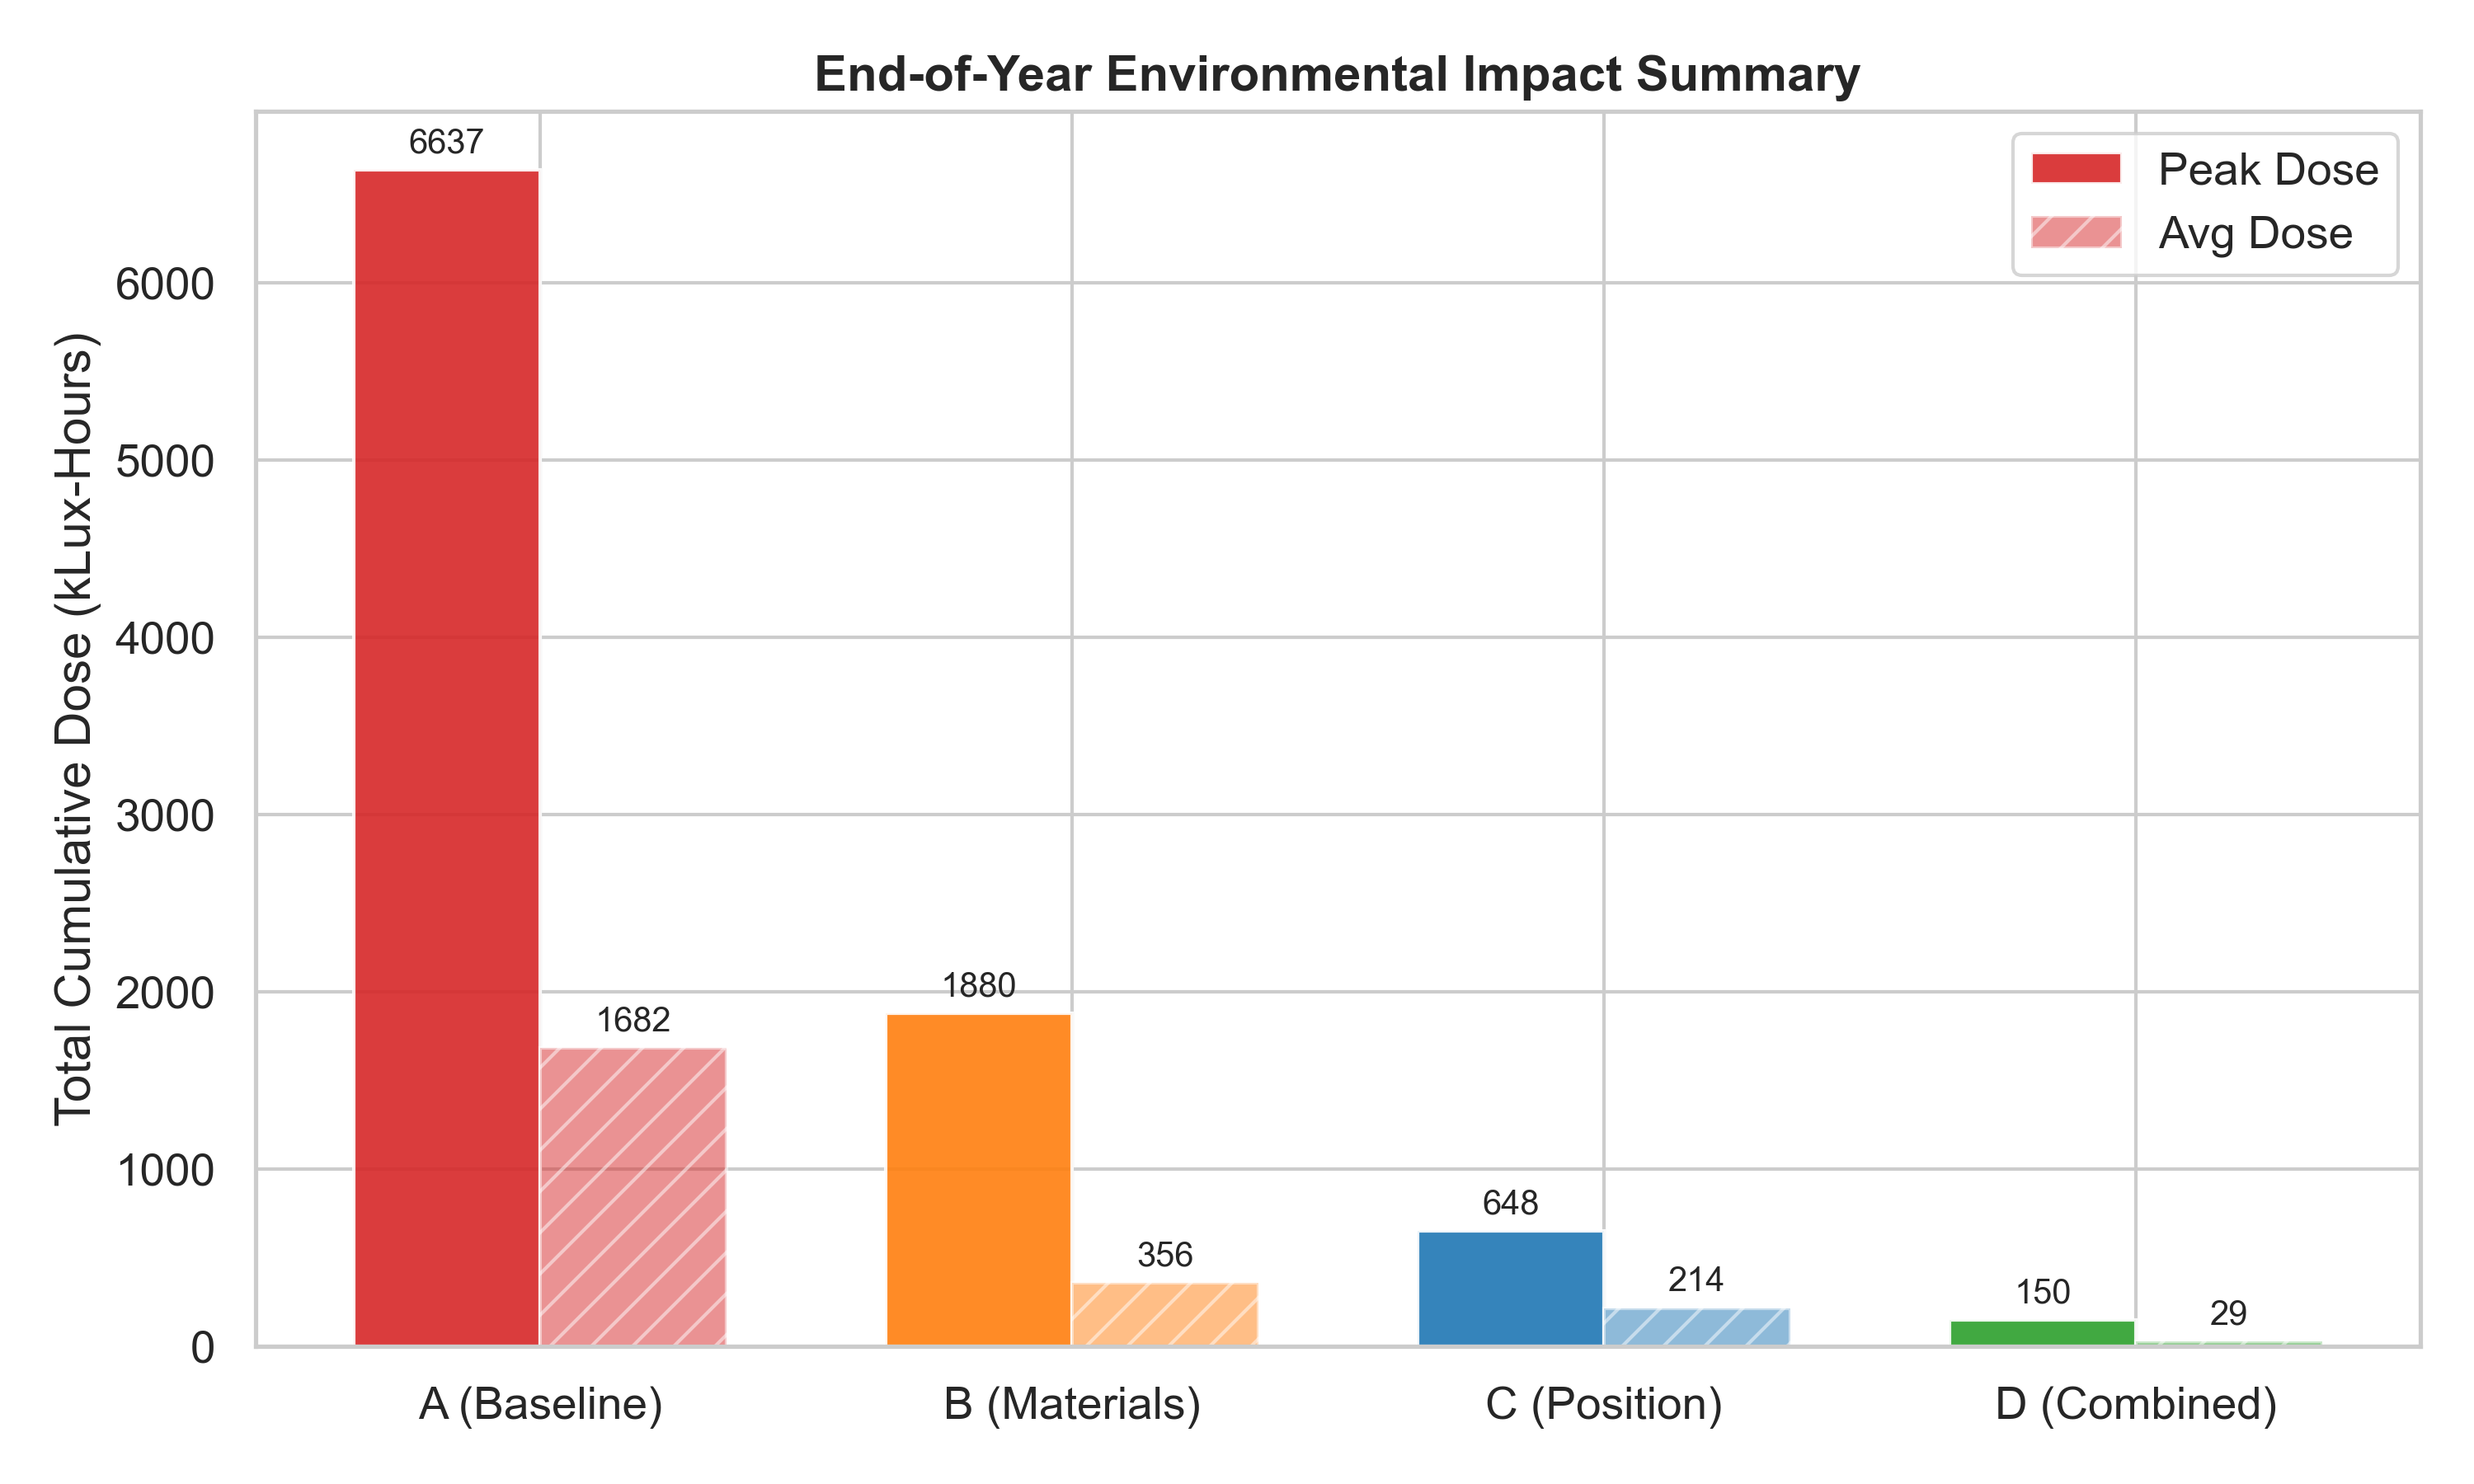
\includegraphics[height=0.6\textheight]{figures/fig2_final_dose_bar.png}
    \vspace{0.5cm}
    \begin{itemize}
        \item \textbf{Massive Reduction:} Scenario D limits the absolute peak to 150k Lux-Hours (a 97.7\% decrease) and average to 28k, making it safe under CIE limits.
    \end{itemize}
\end{frame}

% --- Slide 15: Validation - Spatial Variance ---
\begin{frame}{Scientific Validation: Spatial Variance}
    \centering
    
\includegraphics[height=0.6\textheight]{figures/fig3a_spatial_dose_variance.png}
    \vspace{0.5cm}
    \begin{itemize}
        \item \textbf{Variance Constraint:} Spatial variance scales predictably with physical exposure, demonstrating a mathematically divergent-free integration across the artifact.
    \end{itemize}
\end{frame}

% --- Slide 16: Validation - Sensor Error ---
\begin{frame}{Scientific Validation: Sensor Error}
    \centering
    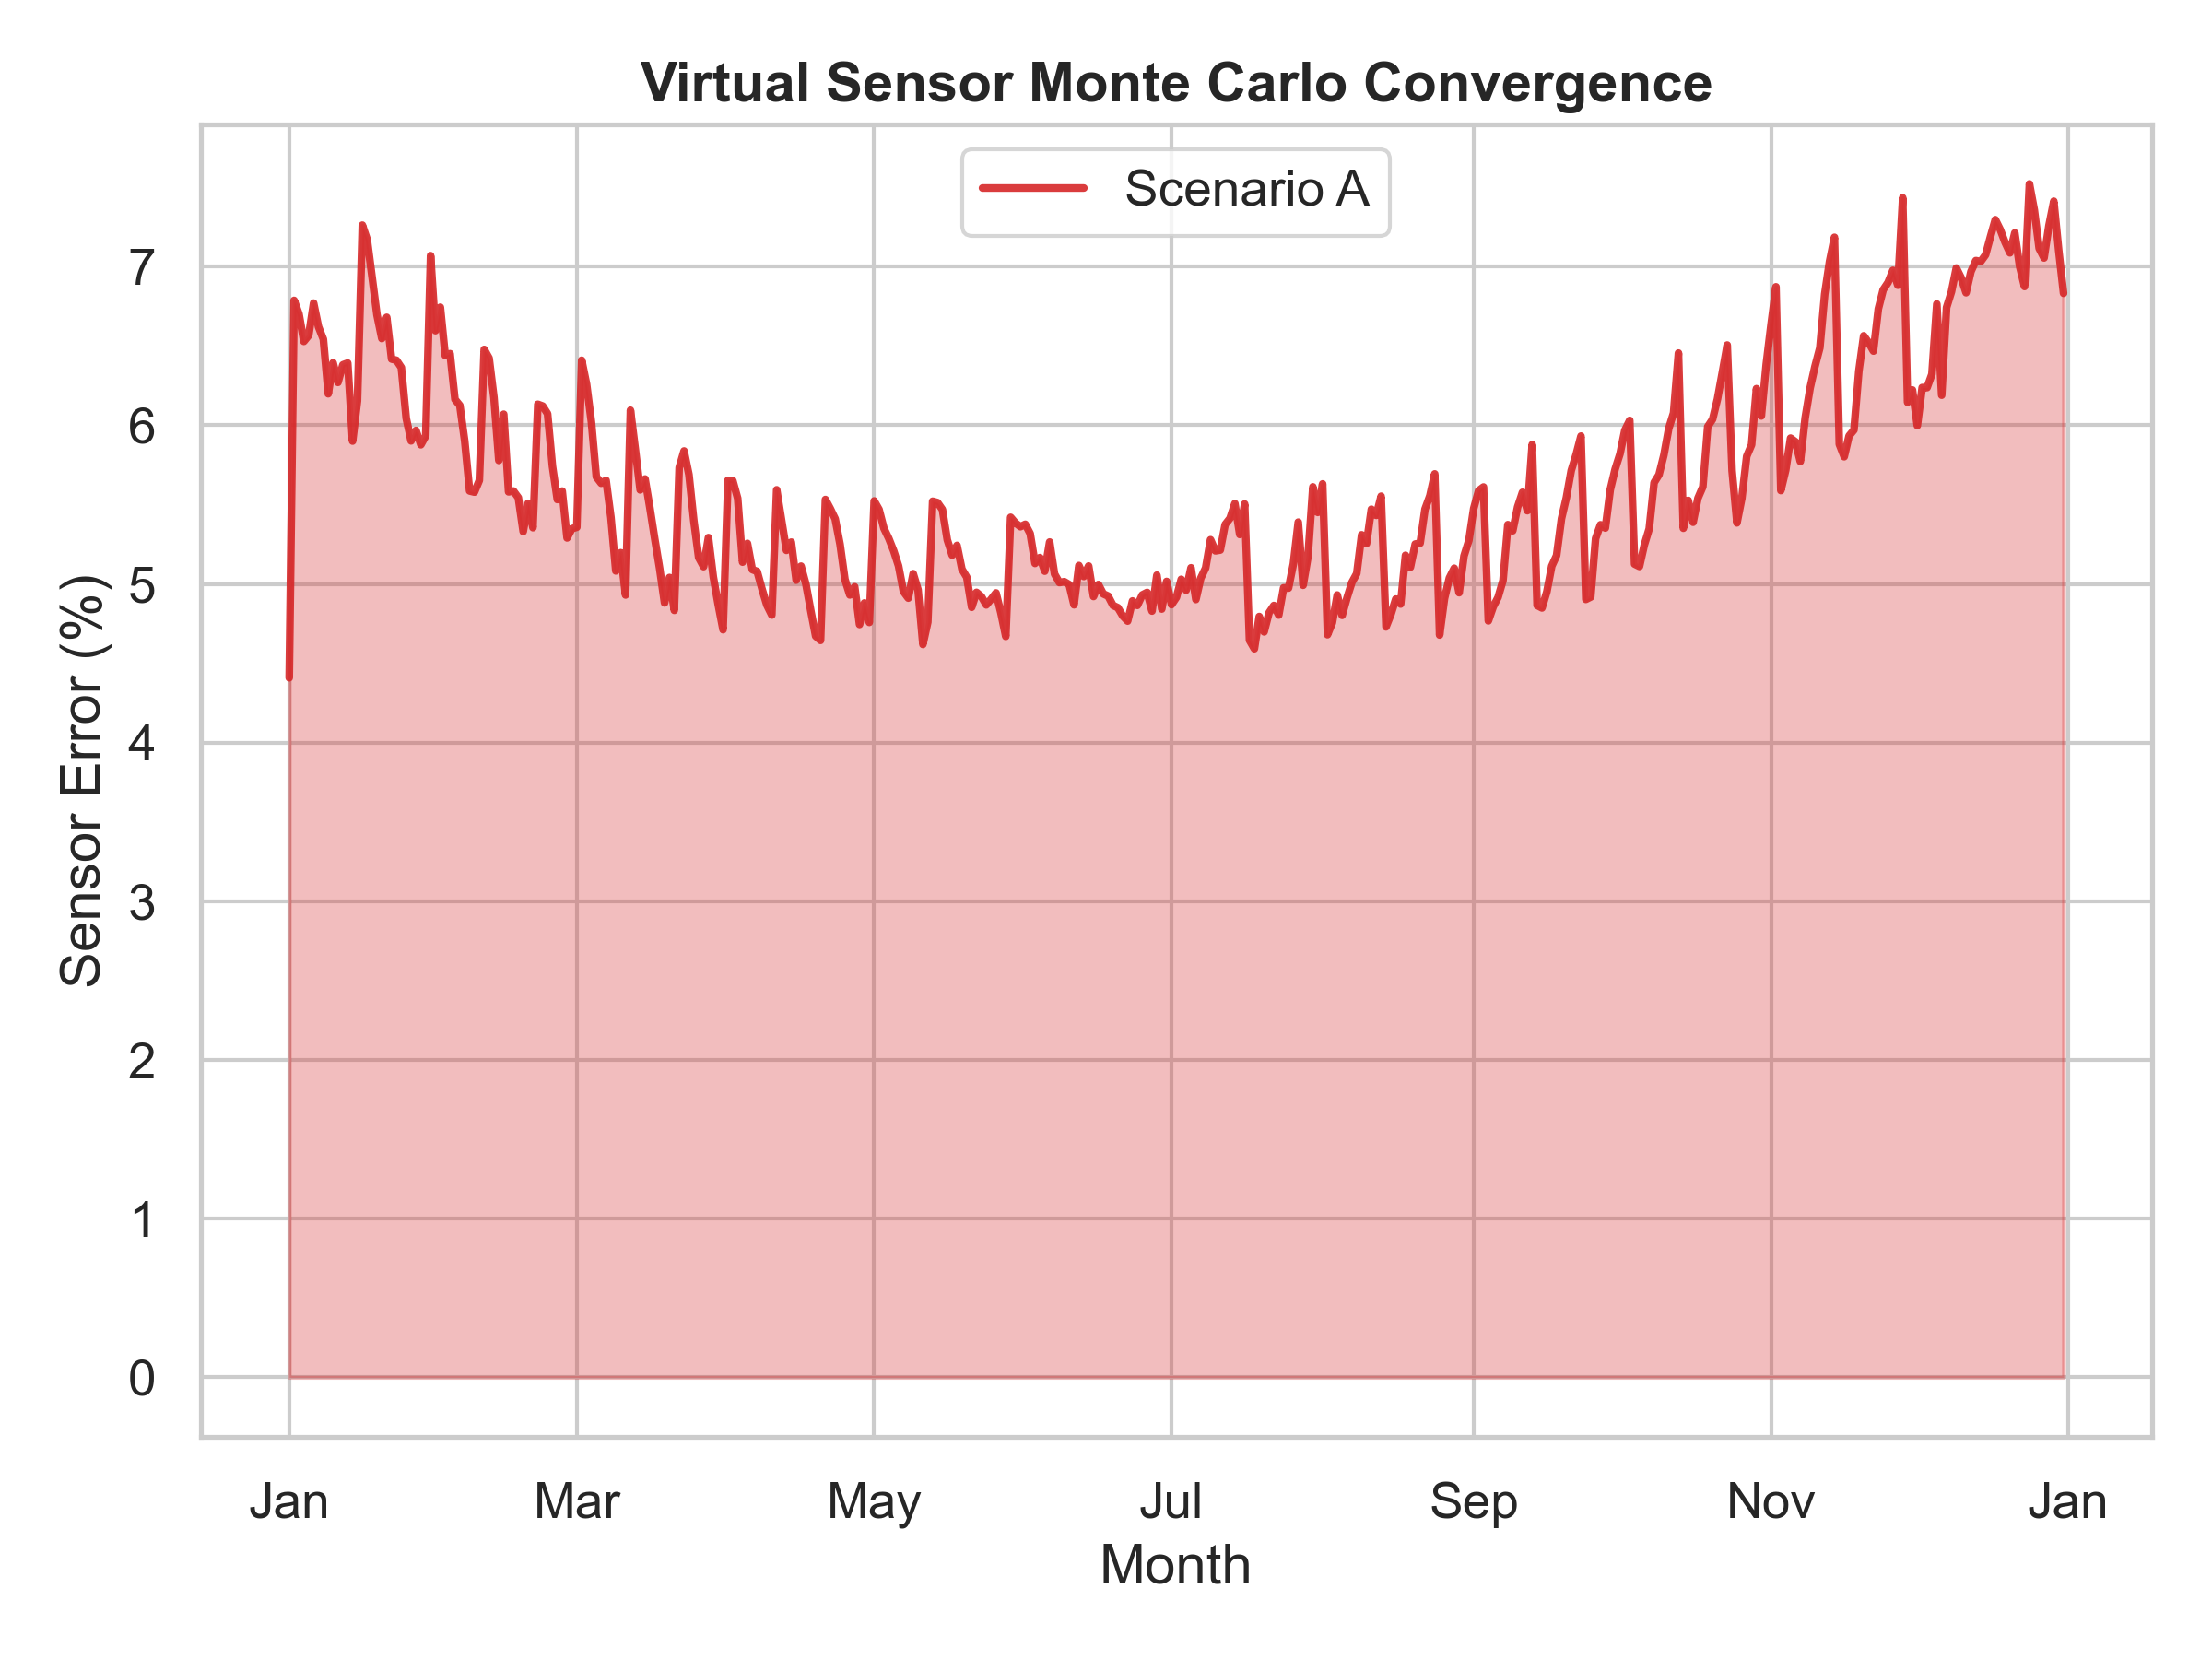
\includegraphics[height=0.6\textheight]{figures/fig3b_monte_carlo_convergence.png}
    \vspace{0.5cm}
    \begin{itemize}
        \item \textbf{Mathematical Reliability:} Stochastic Monte Carlo integration stays strictly bounded to a 4.5\%--7.5\% error margin against deterministic models over 8,760 hours.
    \end{itemize}
\end{frame}

% --- Slide 17: Conclusions ---
\begin{frame}{Conclusions}
    \begin{itemize}
        \item The implementation proves that Texture Space Ray Tracing is a highly viable solution for metrological dosimetry.
        \item Material interventions alone (Scenario B) are insufficient without geometric occlusion (Scenario C).
        \item Digital Twins allow safe, mathematical evaluation of conservation strategies \textbf{before} any physical intervention occurs.
    \end{itemize}
\end{frame}

% --- Slide 18: Bibliography ---
\begin{frame}{Bibliography}
    \begin{thebibliography}{99}
        \setbeamertemplate{bibliography item}[text]
        \bibitem{pharr} M. Pharr, W. Jakob, G. Humphreys, \textit{Physically Based Rendering}, 2016.
        \bibitem{veach} E. Veach, L. J. Guibas, ``Optimally combining sampling techniques'', 1995.
        \bibitem{perez} R. Perez et al., ``All-weather model for sky luminance'', 1993.
    \end{thebibliography}
\end{frame}

\end{document}
